\begin{frame}[fragile]
\frametitle{The introductory example under the \cinkrestrict semantics}
\begin{minted}[escapeinside=||,mathescape=true,texcomments]{c}
// Scope \scope{foo}
int foo(int* restrict p, int* restrict q) {   
    *p = 10;
    *q = 11;
    return *p;
}
\end{minted}

\begin{figure}[h]
\centering
\begin{minipage}{.33\textwidth}
\begin{minted}[escapeinside=||,mathescape=true,texcomments]{c}
// Scope \scope{main}
|\colorbox{red!20}{int main() \{}|
    int x;
    foo(&x, &x);
}
\end{minted}
\end{minipage}%
\begin{minipage}{.67\textwidth}
\executionannotation
{
    $\emptyset$
}
{
    \begin{tikzpicture}[stack/.style={rectangle split, rectangle split parts=#1, draw, anchor=center, text centered},
        scope/.style={fill=gray!20, anchor=center}]
    \node[stack=1, minimum width=4.0cm] (s) {
    \nodepart{one} $\emptyset$
    };
    \node[scope, left=5pt of s.one west]   {\colorbox{red!20}{\scope{main}}};
    \end{tikzpicture}   
}
\end{minipage}
\end{figure}

\end{frame}


% ----

\begin{frame}[fragile]
\frametitle{The introductory example under the \cinkrestrict semantics}
\begin{minted}[escapeinside=||,mathescape=true,texcomments]{c}
// Scope \scope{foo}
int foo(int* restrict p, int* restrict q) {   
    *p = 10;
    *q = 11;
    return *p;
}
\end{minted}

\begin{figure}[h]
\centering
\begin{minipage}{.33\textwidth}
\begin{minted}[escapeinside=||,mathescape=true,texcomments]{c}
// Scope \scope{main}
int main() {
    |\colorbox{red!20}{int x;}| // $\&x = \Blockvar_x$
    foo(&x, &x);
}
\end{minted}
\end{minipage}%
\begin{minipage}{.67\textwidth}
\executionannotation
{
\{\colorbox{red!20}{$\Blockvar_x \mapsto \vundef$}\}
}
{
\begin{tikzpicture}[stack/.style={rectangle split, rectangle split parts=#1, draw, anchor=center, text centered},
        scope/.style={fill=gray!20, anchor=center}]
\node[stack=1, minimum width=4.0cm] (s) {
\nodepart{one} $\emptyset$
};
\node[scope, left=5pt of s.one west]   {\scope{main}};

\end{tikzpicture}
}
\end{minipage}
\end{figure}

\end{frame}


% ----

\begin{frame}[fragile]
\frametitle{The introductory example under the \cinkrestrict semantics}
\begin{minted}[escapeinside=||,mathescape=true,texcomments]{c}
// Scope \scope{foo} \quad $\&p = \Blockvar_p$ \quad $\&q = \Blockvar_q$
int foo(int* restrict p, int* restrict q) { 
    *p = 10;
    *q = 11;
    return *p;
}
\end{minted}

\begin{figure}[h]
\centering
\begin{minipage}{.33\textwidth}
\begin{minted}[escapeinside=||,mathescape=true,texcomments]{c}
// Scope \scope{main}
int main() {
    int x; // $\&x = \Blockvar_x$
    |\colorbox{red!20}{foo(&x, &x);}|
}
\end{minted}
\end{minipage}%
\begin{minipage}{.67\textwidth}
\executionannotation
{
\{\colorbox{red!20}{$\Blockvar_p \mapsto \ptr{(\Blockvar_x, \set{(\Blockvar_p, \scope{foo})})}$},\\
                                            \ \colorbox{red!20}{$\Blockvar_q \mapsto \ptr{(\Blockvar_x, \set{(\Blockvar_q, \scope{foo})})}$}, \\
                                            \ $\Blockvar_x \mapsto \vundef$\}
}
{
\begin{tikzpicture}[stack/.style={rectangle split, rectangle split parts=#1, draw, anchor=center, text centered},
        scope/.style={fill=gray!20, anchor=center}]
\node[stack=2, minimum width=4.0cm] (s) {
    \nodepart{one} $\emptyset$
    \nodepart{two} $\emptyset$
};
\node[scope, left=5pt of s.one west]   {\colorbox{red!20}{\scope{foo}}};
\node[scope, left=5pt of s.two west]   {\scope{main}};

\end{tikzpicture}
}
\end{minipage}
\end{figure}
\end{frame}

% ----

\begin{frame}[fragile]
\frametitle{The introductory example under the \cinkrestrict semantics}
\begin{minted}[escapeinside=||,mathescape=true,texcomments]{c}
// Scope \scope{foo} \quad $\&p = \Blockvar_p$ \quad $\&q = \Blockvar_q$
int foo(int* restrict p, int* restrict q) {   
    |\colorbox{red!20}{*p = 10;}|
    *q = 11;
    return *p;
}
\end{minted}

\begin{figure}[h]
\centering
\begin{minipage}{.33\textwidth}
\begin{minted}[escapeinside=||,mathescape=true,texcomments]{c}
// Scope \scope{main}
int main() {
    int x; // $\&x = \Blockvar_x$
    foo(&x, &x);
}
\end{minted}
\end{minipage}%
\begin{minipage}{.67\textwidth}
\executionannotation
{\{$\Blockvar_p \mapsto \ptr{(\Blockvar_x, \set{(\Blockvar_p, \scope{foo})})}$,\\
                                            \ $\Blockvar_q \mapsto \ptr{(\Blockvar_x, \set{(\Blockvar_q, \scope{foo})})}$, \\
                                            \ $\Blockvar_x \mapsto \colorbox{red!20}{10}$\}
}
{
\begin{tikzpicture}[stack/.style={rectangle split, rectangle split parts=#1, draw, anchor=center, text centered},
        scope/.style={fill=gray!20, anchor=center}]
% Stack
\node[stack=2, minimum width=4.0cm] (s) {
    \nodepart{one} \{\colorbox{red!20}{$\Blockvar_x \mapsto \restricted{\set{(\Blockvar_p, \scope{foo})}}$}\}
    \nodepart{two} $\emptyset$
};

% Scopes
\node[scope, left=5pt of s.one west]   {\scope{foo}};
\node[scope, left=5pt of s.two west]   {\scope{main}};

\end{tikzpicture}
}
\end{minipage}
\end{figure}

\end{frame}


% ----

\begin{frame}[fragile]
\frametitle{The introductory example under the \cinkrestrict semantics}
\begin{minted}[escapeinside=||,mathescape=true,texcomments]{c}
// Scope \scope{foo} \quad $\&p = \Blockvar_p$ \quad $\&q = \Blockvar_q$
int foo(int* restrict p, int* restrict q) {   
    *p = 10;
    |\colorbox{red!20}{*q = 11;}|
    return *p;
}
\end{minted}
\vspace*{-30pt}
\begin{figure}[h]
\centering
\begin{minipage}{.33\textwidth}
\begin{minted}[escapeinside=||,mathescape=true,texcomments]{c}
// Scope \scope{main}
int main() {
    int x; // $\&x = \Blockvar_x$
    foo(&x, &x);
}
\end{minted}
\end{minipage}%
\begin{minipage}{.67\textwidth}
\colorbox{red!20}{$\restricted{\set{(\Blockvar_\text{\textcolor{blue}{$q$}}, \scope{foo})}} \joinsym \restricted{\set{(\Blockvar_\text{\textcolor{blue}{$p$}}, \scope{foo})}} = ...$}
\\

\executionannotation
{\{$\Blockvar_p \mapsto \ptr{(\Blockvar_x, \set{(\Blockvar_p, \scope{foo})})}$,\\
                                            \ $\Blockvar_q \mapsto \ptr{(\Blockvar_x, \set{(\Blockvar_q, \scope{foo})})}$, \\
                                            \ $\Blockvar_x \mapsto \vundef$\}
}
{
\begin{tikzpicture}[stack/.style={rectangle split, rectangle split parts=#1, draw, anchor=center, text centered},
        scope/.style={fill=gray!20, anchor=center}]
% Stack
\node[stack=2, minimum width=4.0cm] (s) {
    \nodepart{one} $\set{\Blockvar_x \mapsto \restricted{\set{(\Blockvar_p, \scope{foo})}}}$
    \nodepart{two} $\emptyset$
};

% Scopes
\node[scope, left=5pt of s.one west]   {\scope{foo}};
\node[scope, left=5pt of s.two west]   {\scope{main}};

\end{tikzpicture}
}
\end{minipage}
\end{figure}

\end{frame}




% ----

\begin{frame}[fragile]
\frametitle{The introductory example under the \cinkrestrict semantics}
\colorbox{red!20}{$\restricted{\set{(\Blockvar_\text{\textcolor{blue}{$q$}}, \scope{foo})}} \joinsym \restricted{\set{(\Blockvar_\text{\textcolor{blue}{$p$}}, \scope{foo})}} = ...$}

\begin{minipage}{.5\textwidth}
\begin{itemize}
    \item The symmetric \joinsym \ operation describes the result of joining two restrict states \\~\\
    \item \footnotesize$\unresabbr = \unrestricted$, $\resabbr{\Basesvar} = (\restricted{\Basesvar})$ and $\orabbr{\Basesvar} = (\onlyread{\Basesvar})$
    \item \footnotesize$\Basesvar \neq \Basesvar'$
\end{itemize}
\end{minipage}%
\begin{minipage}{.5\textwidth}

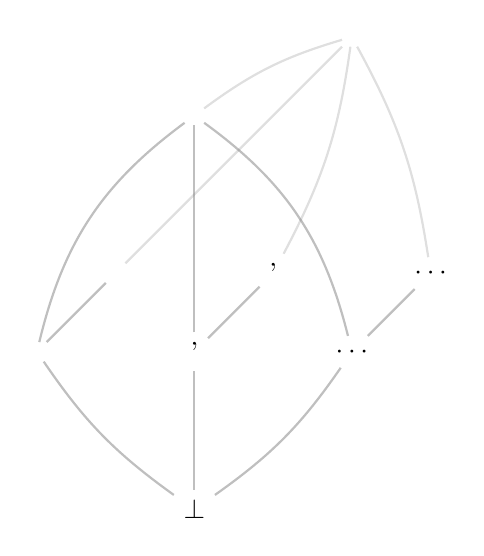
\begin{tikzpicture}
    \node (ub)     at (7,5) {\rsub};
    \node (un)     at (5,4) {\unresabbr};
    \node (rsbs)   at (4,2) {\resabbr{\Basesvar}};
    \node (rsbs')  at (6,2) {\resabbr{\Basesvar'}};
    \node (rsbs'') at (8,2) {$\cdots$};
    \node (orbs)   at (3,1) {\orabbr{\Basesvar}};
    \node (orbs')  at (5,1) {\orabbr{\Basesvar'}};
    \node (orbs'') at (7,1) {$\cdots$};
    \node (bot)    at (5,-1) {$\bot$};

    \path[thick, black, opacity=0.25]
    (bot) edge[bend left=10] node {} (orbs)
    (bot) edge node {} (orbs')
    (bot) edge[bend right=10] node {} (orbs'')
    
    (orbs) edge node {} (rsbs) 
    (orbs') edge node {} (rsbs')
    (orbs'') edge node {} (rsbs'')  
    
    (orbs) edge[bend left=20] node {} (un)
    (orbs') edge node {} (un)
    (orbs'') edge[bend right=20] node {} (un)

    (rsbs) edge[gray] node {} (ub)
    (rsbs') edge[bend right=10, gray] node {} (ub)
    (rsbs'') edge[bend right=10, gray] node {} (ub)

    (un) edge[bend left=10, gray] node {} (ub);
\end{tikzpicture}
\end{minipage}

\end{frame}


% ----

\begin{frame}[fragile]
\frametitle{The introductory example under the \cinkrestrict semantics}

\colorbox{red!20}{$\restricted{\set{(\Blockvar_\text{\textcolor{blue}{$q$}}, \scope{foo})}} \joinsym \restricted{\set{(\Blockvar_\text{\textcolor{blue}{$p$}}, \scope{foo})}} = \rsub$}

\begin{minipage}{.5\textwidth}
\begin{itemize}
    \item The symmetric \joinsym \ operation describes the result of joining two restrict states \\~\\
    \item \footnotesize$\unresabbr = \unrestricted$, $\resabbr{\Basesvar} = (\restricted{\Basesvar})$ and $\orabbr{\Basesvar} = (\onlyread{\Basesvar})$
    \item \footnotesize$\Basesvar \neq \Basesvar'$
\end{itemize}
\end{minipage}%
\begin{minipage}{.5\textwidth}

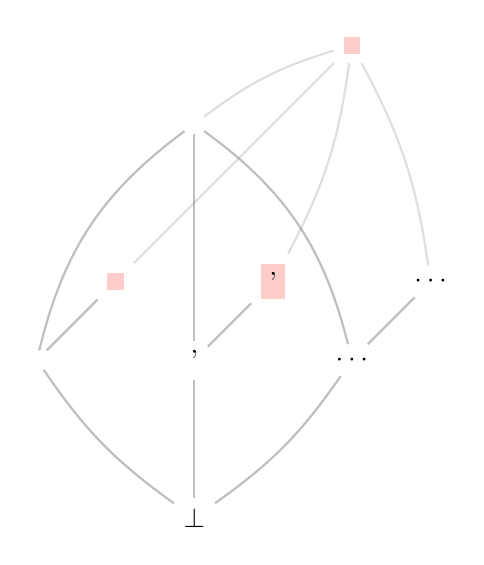
\begin{tikzpicture}
    \node (ub)     at (7,5) {\colorbox{red!20}{\rsub}};
    \node (un)     at (5,4) {\unresabbr};
    \node (rsbs)   at (4,2) {\colorbox{red!20}{\resabbr{\Basesvar}}};
    \node (rsbs')  at (6,2) {\colorbox{red!20}{\resabbr{\Basesvar'}}};
    \node (rsbs'') at (8,2) {$\cdots$};
    \node (orbs)   at (3,1) {\orabbr{\Basesvar}};
    \node (orbs')  at (5,1) {\orabbr{\Basesvar'}};
    \node (orbs'') at (7,1) {$\cdots$};
    \node (bot)    at (5,-1) {$\bot$};

    \path[thick, black, opacity=0.25]
    (bot) edge[bend left=10] node {} (orbs)
    (bot) edge node {} (orbs')
    (bot) edge[bend right=10] node {} (orbs'')
    
    (orbs) edge node {} (rsbs) 
    (orbs') edge node {} (rsbs')
    (orbs'') edge node {} (rsbs'')  
    
    (orbs) edge[bend left=20] node {} (un)
    (orbs') edge node {} (un)
    (orbs'') edge[bend right=20] node {} (un)

    (rsbs) edge[gray] node {} (ub)
    (rsbs') edge[bend right=10, gray] node {} (ub)
    (rsbs'') edge[bend right=10, gray] node {} (ub)

    (un) edge[bend left=10, gray] node {} (ub);
\end{tikzpicture}
\end{minipage}

\end{frame}

% ----

\begin{frame}[fragile]
\frametitle{The introductory example under the \cinkrestrict semantics}
\begin{minted}[escapeinside=||,mathescape=true,texcomments]{c}
// Scope \scope{foo} \quad $\&p = \Blockvar_p$ \quad $\&q = \Blockvar_q$
int foo(int* restrict p, int* restrict q) {   
    *p = 10;
    |\colorbox{red!20}{*q = 11;}|
    return *p;
}
\end{minted}
\vspace*{-30pt}
\begin{figure}[h]
\centering
\begin{minipage}{.33\textwidth}
\begin{minted}[escapeinside=||,mathescape=true,texcomments]{c}
// Scope \scope{main}
int main() {
    int x; // $\&x = \Blockvar_x$
    foo(&x, &x);
}
\end{minted}
\end{minipage}%
\begin{minipage}{.67\textwidth}
\textbf{UB}: \colorbox{red!20}{$\restricted{\set{(\Blockvar_\text{\textcolor{blue}{$q$}}, \scope{foo})}} \joinsym \restricted{\set{(\Blockvar_\text{\textcolor{blue}{$p$}}, \scope{foo})}} = \rsub$}
\\

\executionannotation
{\{$\Blockvar_p \mapsto \ptr{(\Blockvar_x, \set{(\Blockvar_p, \scope{foo})})}$,\\
                                            \ $\Blockvar_q \mapsto \ptr{(\Blockvar_x, \set{(\Blockvar_q, \scope{foo})})}$, \\
                                            \ $\Blockvar_x \mapsto \vundef$\}
}
{
\begin{tikzpicture}[stack/.style={rectangle split, rectangle split parts=#1, draw, anchor=center, text centered},
        scope/.style={fill=gray!20, anchor=center}]
% Stack
\node[stack=2, minimum width=4.0cm] (s) {
    \nodepart{one} $\set{\Blockvar_x \mapsto \restricted{\set{(\Blockvar_p, \scope{foo})}}}$
    \nodepart{two} $\emptyset$
};

% Scopes
\node[scope, left=5pt of s.one west]   {\scope{foo}};
\node[scope, left=5pt of s.two west]   {\scope{main}};

\end{tikzpicture}
}
\end{minipage}
\end{figure}

\end{frame}
